\documentclass[12pt]{article}

\usepackage{formatting}
\usepackage{tikz}

\usetikzlibrary{shapes.geometric, arrows}
\tikzstyle{startstop} = [rectangle, rounded corners, minimum width=3cm, minimum height=1cm,text centered, draw=black, fill=red!30]
\tikzstyle{io} = [trapezium, trapezium left angle=70, trapezium right angle=110, minimum width=3cm, minimum height=1cm, text centered, text width=3cm, draw=black, fill=blue!30]
\tikzstyle{process} = [rectangle, minimum width=3cm, minimum height=1cm, text centered, text width=3.5cm, draw=black, fill=orange!30]
\tikzstyle{decision} = [diamond, minimum width=3cm, minimum height=1cm, text centered, text width=3cm, draw=black, fill=green!30]
\tikzstyle{arrow} = [thick,->,>=stealth]

% Use https://uwaterloo.ca/math/current-undergraduates/co-op-information/work-report-guidelines/appendix-3-work-report-checklist to ensure you are meeting all the requirements

%%%%%%%%%%%%%%%%%%%%%%%%%%%%%%%%%%%

% Fill in:

%%%%%%%%%%%%%%%%%%%%%%%%%%%%%%%%%%%


\newcommand{\term}{1B } % term that was most recently completed
\newcommand{\program}{Computing and Financial Management}
\newcommand{\WTT}{Pursuing Further Automation in Data Collection}
\newcommand{\name}{Timothy Zheng}
\newcommand{\studentNumber}{XXXXXX}

\newcommand{\yourStreet}{Street}
\newcommand{\yourCity}{City}
\newcommand{\yourProvince}{ Province}
\newcommand{\yourPostalCode}{Postal Code}

\newcommand{\supervisorsName}{TBD}
\newcommand{\supervisorsRole}{PD 11 Evaluators}

\newcommand{\compName}{Advanced Micro Devices (AMD)}
\newcommand{\compStreet}{1 Commerce Valley Dr E}
\newcommand{\compCity}{Thornhill}
\newcommand{\compProvince}{ON}
\newcommand{\compPostalCode}{L3T 7X6}

\begin{document}

%%%%%%%%%%%%%%%%%%%%%%%%%%%%%%%%%%%

% Title Page:

%%%%%%%%%%%%%%%%%%%%%%%%%%%%%%%%%%%


\FirstPage

\newpage

%%%%%%%%%%%%%%%%%%%%%%%%%%%%%%%%%%%

% Letter:

%%%%%%%%%%%%%%%%%%%%%%%%%%%%%%%%%%%

%\LetterHead
%
%% Sample is at https://uwaterloo.ca/math/sites/ca.math/files/uploads/files/letterofsubmittal_2.pdf"
%
%
%As we agreed, I have prepared the enclosed report, “\WTT,” for
%my \term work report and for the TEAM. This
%report, the first of four work reports that the Co-operative Education Program
%requires that I successfully complete as part of my BMath Co-op degree
%requirements, has not received academic credit.
%\vskip 10pt
%ROLE IN COMPANY, BRIEF DESCRIPTION OF DUTIES, PURPOSE OF REPORT must be added in a paragraph
%\vskip 10pt 
%The Faculty of Mathematics requests that you evaluate this report for command
%of topic and technical content/analysis. Following your assessment, the report,
%together with your evaluation, will be submitted to the Math Undergrad Office
%for evaluation on campus by qualified work report markers. The combined
%marks determine whether the report will receive credit and whether it will be
%considered for an award.
%\vskip 10pt 
%Thank you for your assistance in preparing this report.
%
%Timothy Zheng
%
%% \includegraphics[height=3cm]{Signature.jpg}


%%%%%%%%%%%%%%%%%%%%%%%%%%%%%%%%%%%

% Table of Contents:

%%%%%%%%%%%%%%%%%%%%%%%%%%%%%%%%%%%

\toc 

%%%%%%%%%%%%%%%%%%%%%%%%%%%%%%%%%%%

\sectionNoNumber{Executive Summary}

% Complete clear well organized summary of 1) the purpose of the report, 2) key points of analysis and highlights the conclusion

%%%%%%%%%%%%%%%%%%%%%%%%%%%%%%%%%%%


% One of the most important components of the report is the Executive Summary. It should be written after the rest of the report has been written.

% The Executive Summary should be complete in itself and may be consulted by readers to determine whether they need to read the whole report. It appears on a separate page.

% Limit the Executive Summary to one page and briefly present

% the purpose of the report
% the key points of the analysis
% the highlights of the conclusions
% the highlights of the recommendations

\indent\hspace{0.5in} The collection and processing of performance data is a vital asset in the manufacturing of modern computer microprocessors. Advanced Micro Devices (AMD) uses this data to better understand their products throughout the development process and market their products to end users. Data is collected on popular software products used by AMD's customers with the help of a computer-automated program that must be maintained by a team of lab technicians. This report investigates potential areas of the data collection workflow where processes could be further optimized using computer technology. The two tasks that are being considered are

\begin{enumerate}
\item Improving data ingestion using a novel software interface.
\item Automatically generating data presentation and processing spreadsheets.
\end{enumerate}

\indent\hspace{0.5in} Both solutions showcase that the bottleneck in the data collection process occurs when raw data has to be ingested into Microsoft Excel spreadsheets for further processing before being presented to internal data customers. Neither solutions are simple to implement, and will require some investment before they begin to show positive returns in improved productivity. By considering these methods, it is clear that there are smaller areas where improvements could be implemented at a smaller, but more time-effective manner. By increasing the degree of automation of monotonous tasks in the workplace, the report finds that worker satisfaction and productivity increases as a result of the increased amount of time workers have to make dynamic, thought-provoking decisions.

%%%%%%%%%%%%%%%%%%%%%%%%%%%%%%%%%%%

\formattingForRestOfReport
\section{Introduction}

%%%%%%%%%%%%%%%%%%%%%%%%%%%%%%%%%%%


% The Introduction establishes the purpose of the report and conveys the contents of the Analysis. You should provide the reader with the following information:

% necessary background information
% assumptions used
% major points covered in the report
% the situation or problem that is analyzed
% the purpose of the work report and the methodology used


\indent\hspace{0.5in} The purpose of this report is to explore areas in which procedures for data-collection and test coordination could be optimized, and discuss the tradeoff between time invested and time saved in the process of developing and implementing computer-assisted automation scripts in selected areas.  

\indent\hspace{0.5in} Advanced Micro Devices (AMD) is an American semiconductor company focused on producing high-performance processor technologies for the most demanding use-cases in the modern era (AMD, nd). AMD’s portfolio of leading-edge semiconductor products such as CPUs, GPU, FPGAs, and Adaptive SoCs can be found in a broad range of products ranging from consumer electronics such as personal computers (PCs), laptops, current-generation gaming consoles and electric vehicles to enterprise and government deployments of supercomputers that seek to uncover the next leap in meteorological, artificial intelligence, and theoretical physics research (AMD). 

\indent\hspace{0.5in} In producing these products, AMD requires an extensive understanding on the performance of their products throughout the development cycle. Performance data provides feedback to various internal teams to ensure performance goals are met and identify areas of improvement. Moreover, data gathered on products near the end of their development timeline is used to prepare marketing assets which are presented to AMD’s business partners, or to consumers directly through trade shows and advertisements. In the latter case, performance data is gathered in end-user programs such as popular video games. 
This report will focus on the exploration of areas in which automation may be implemented or improved in workflows revolving around performance testing on consumer notebook products near the end of their development timelines. Automation takes simple, rudimentary tasks and digitizes work through the use of tools to streamline and centralize routine tasks (IBM, n.d.).



%%%%%%%%%%%%%%%%%%%%%%%%%%%%%%%%%%%
\newpage
\section{Analysis} 

%%%%%%%%%%%%%%%%%%%%%%%%%%%%%%%%%%%

\subsection{Understanding Computer Automation}
\indent\hspace{0.5in} With the rapid pace of technological adoption in the workplace, it seems like a no-brainer for companies and teams to start incorporating digitally aided automation technologies into their daily workflows. Companies that integrate digital technologies in their workflows provide their employees with a more enriched work balance because workers are given the autonomy and space for self-development. Workers transition from performing monotonous tasks to becoming strategic decision-makers and flexible problem-solvers (Leesakul, et al., 2022). The challenges which the author of the report faces in the workplace heavily center around working with repetitive data-heavy tasks such as data ingestion and processing, and can be accelerated exponentially through computer-aided scripts. To provide some context, this problem is far from being isolated in the data sector - "In fact, research indicates that nearly 70\% of business processes that could be automated are still manual" (Fleckenstein et. al., 2018, para. 2). The first step to tackling this problem is to identify areas of repetitive, and easily optimized workflows. Once they are found, algorithms and machine intelligence are implemented, speeding up tasks, and eliminating human-error in monotonous tasks, at which point computers are able to identify potential errors and flag them for human review (Fleckenstein et. al.).  Cummings et al. (2016) discovered that bright and diligent workers quickly become overwhelmed by tasks that require constant attention and lack dynamism. In reality, tasks such as data collection do require constant attention in case of errors that can break any ongoing collection task, but is incredibly lackluster to observe for long periods of time. Ideally, it would be much easier, and less straining on skilled workers if it was possible for computer intelligence to notify a human only if there is a problem, at which point the worker can use their skills to address and fix the problem. While the automation program is observing data collection tasks, the human worker can spend their time adapting the program to work better, or improve efficiencies elsewhere, ultimately improving worker satisfaction and net useful output. 

\subsubsection{Cost-benefit Analysis}
\indent\hspace{0.5in} It is also important to understand the limitations in working hours and scheduling that arise in the job. It is difficult, and often unreasonable to for example, set aside two hours of the working day attempting to automate a task that may only be used once or twice and is quicker to be done manually. In order to create a program that could be used universally, a more dedicated approach must be taken, which consumes more time upfront and for the scope of a 4-month co-op placement, may not see use until near the end of the work term, at which point the tool may be deprecated when presented to the next batch of co-ops working at the same department. Indeed, primary research in this shows that many scripts attempting to automate monotonous tasks in data collection exist in the team's archives, but many appear to be convoluted, and lack documentation to the point where it is often difficult to figure out what they do, nevertheless the procedure on how to use them. 

\indent\hspace{0.5in} Continuing with viewing the problem of repetitive work in new student hires, Shikdar, et al. (2003) were able to show that workplace satisfaction had a strong positive correlation to productivity. A student would be able to perform better if they were given the option to shift from monotonous tasks to another more thought-provoking assignment. By maintaining workplace morale, the team may not suffer as harshly in the interim period of training new hires every four months, as the team constantly hires new students in this time cycle.

\indent\hspace{0.5in} Therefore, it is possibly a more practical endeavour for students in shorter-term placements to go after tasks building solutions with smaller time horizons that can be tackled as a side-project, or during lulls in the team's testing bandwidth. These tasks can be identified through a quick spot-check where if the task could be automated quicker than the time it takes for the task to be done manually once, then automating such tasks may be something worth pursuing. Once the script for that simple task is built, it may be polished as it is used more, producing a structure for maturing code the more it is used, and leaving ad hoc tasks where an automated script is only required once to be left in its simple form. Wider-scope projects may be considered by senior members of the team to implement with permanent members.

\subsubsection{Approach}
\indent\hspace{0.5in} A methodical approach is taken to systematically identify areas for improvement. After reviewing each section of the normal handling of one of the laptops through each stage of the data collection process, it is apparent that the majority of the “low-hanging fruit” present occurs in the data collection and presentation process. That is, by picking tasks that have short fixes, but large time-efficiency implications should be worked at first due to them being valued the best, when considering workers' time as the most important asset. Due to the structure of the regular 9 to 5 workday, it is impractical to optimize the installation of prerequisite software, as it is often too dynamic to be reliably automated without unjustifiably high amounts of overhead and sunk costs. To this end, it is also impractical to automate the ingestion of prototype testing platforms near the head-end of the testing cycle, as it requires a high degree of discussion, planning and logistics work that is best done by humans. These tasks do not align with the issues presented by Cummings et al. (2016) in their report, as these tasks require lots of problem-solving, communication, creativity and dynamism that rule them out of being possibilities for automation. A summary view of a typical workflow through the data collection process is described in Figure 1 below.

\begin{figure}[h!]
\begin{center}
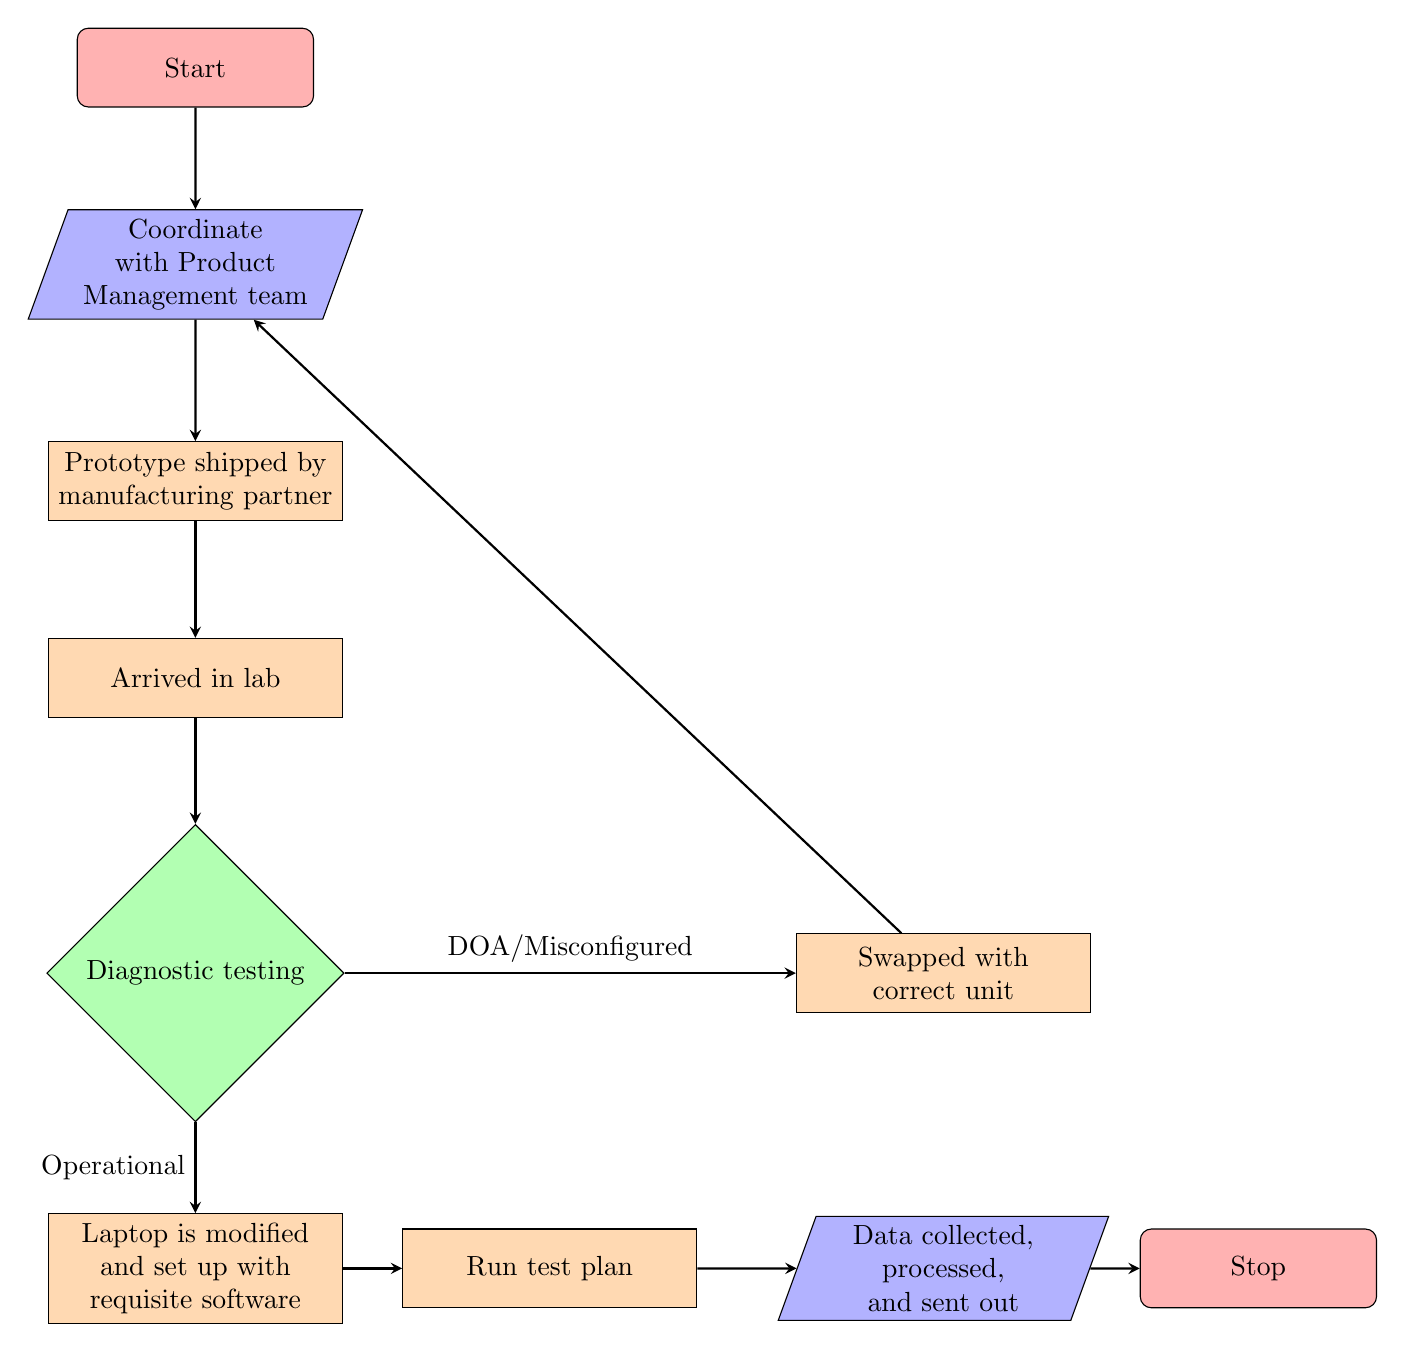
\begin{tikzpicture}[node distance=2cm]
\node (start) [startstop] {Start};
\node (in1) [io, below of=start, yshift=-0.5cm] {Coordinate with Product Management team};
\node (pro1) [process, below of=in1, yshift=-0.75cm] {Prototype shipped by manufacturing partner};
\node (pro2) [process, below of=pro1, yshift=-0.5cm] {Arrived in lab};
\node (dec1) [decision, below of=pro2, yshift=-1.75cm] {Diagnostic testing};
\node (pro3a) [process, below of=dec1, yshift=-1.75cm] {Laptop is modified and set up with requisite software};
\node (pro3b) [process, right of=dec1, xshift=7.5cm] {Swapped with correct unit};
\node (pro4) [process, right of=pro3a, xshift=2.5cm] {Run test plan};
\node(out1) [io, right of=pro4, xshift=3cm] {Data collected, processed, and sent out};
\node (stop) [startstop, right of=out1, xshift=2cm] {Stop};

\draw [arrow] (start) -- (in1);
\draw [arrow] (in1) -- (pro1);
\draw [arrow] (pro1) -- (pro2);
\draw [arrow] (pro2) -- (dec1);
\draw [arrow] (dec1) -- node[anchor=east] {Operational} (pro3a);
\draw [arrow] (dec1) -- node[anchor=south] {DOA/Misconfigured} (pro3b);
\draw [arrow] (pro3b) -- (in1);
\draw [arrow] (pro3a) -- (pro4);
\draw [arrow] (pro4) -- (out1);
\draw [arrow] (out1) -- (stop);

\end{tikzpicture}
\end{center}
\caption{A typical data collection workflow}
\end{figure}
\newpage

\indent\hspace{0.5in} Processes in the tail-end of the process outlined in Figure 1 offer many more tasks that could be classified as “repetitive and lacking in dynamism,” and are in their nature extremely tedious and time-consuming. This area is therefore ripe for improvements in time and talent utilization. In particular, two areas of interest may produce the most benefit for the amount of dedication required to produce a script to adapt them. If designed correctly, these programs are within the job requirements and if properly documented, could be passed along to future employees with little overhead and learning curve. 

\subsection{Approaching Potential Solutions}

\indent\hspace{0.5in} The spreadsheet is a powerful data-packaging tool that is widely distributable throughout the company, and can be easily interpreted and accessed as required. It is incredibly important for internal stakeholders to have an instantaneous and overarching view into the company's product segments, and is a potential rebuttal against transitioning the team to a more modern data distribution system that may require more technical knowledge. Indeed, spreadsheet programs such as Microsoft Excel offer advanced features that may be used by the data-packaging side of the company, internal end-users may never face such controls, and would rather have a read-only view into reports generated using Microsoft Excel. Pemberton, et al (2000) discovers that many corporate employees will at least have some low-level understanding of a spreadsheet program, and will have little trouble interpreting data presented in this form factor. The current data collection program is therefore tailored to generate data which is easily imported into spreadsheets for easy data analytics using Microsoft Excel.

\subsubsection{Improving Data Ingestion}

\indent\hspace{0.5in} Currently, the procedure to ingest data from the team’s proprietary game automation program is to manually read and surgically copy-paste successful runs into a central spreadsheet for further data processing. Since certain runs will fail due to a variety of factors that must be individually diagnosed, it is not simple to select an entire range of cells. On average, this process consumes anywhere from 45 minutes to one hour per machine. By matching entries to data points, a simple program could feasibly select just the runs with data and insert them into the spreadsheet in a split-second. Erroneous data points could be then identified and reported to the user for easy re-runs once the underlying problem has been identified and fixed. It can be foreseen that however, such a program will severely dissuade users from proof-reading the processed results and place their faith entirely in the reliability of the program. Unforeseen errors, or readings populated with data, but containing erroneous data, could slip through the human review once the data ingestion process is completed. The development of such a program will require extensive testing, checks and disclaimers when used, but should significantly accelerate what is the largest bottleneck in the process. This task most strongly meets the criteria laid out by Cummings et al. (2016) to be automated due to its tedious and lacklustre style, and at face-value appears to have the most promising feasibility to be implemented. The results file produced by the existing testing automation script contains all of the required information to quickly and easily match with entries in the central data processing spreadsheet.

\subsubsection{Automatically Generating Data Processing and Presentation Spreadsheets}
\indent\hspace{0.5in} When presenting data to data customers for use in product marketing materials, statistical factors need to considered regarding the use of the numbers the lab produces. That is, due to the significant degree of complication of modern processors, run-to-run variance between results is not trivial. It is important to note that at the end of the day, the goal of the testing results is to demonstrate what a typical customer using one of the tested products may expect in a typical workload. It is therefore necessary to run tests multiple times in order to capture this statistical variance and further process the data points to generate a final result that can be then used by the team's data customers. This process is standard in the industry, and is a necessary step to collecting reputable performance data. Burke, S. (2018) collected data showing this phenomenon on a significant number of consumer computer platforms, proving that it is still an issue across the board with AMD, and its competitors. Steve is a highly trusted figure in technical reporting for the consumer computer segment, whose work directly influences testing standards and methodology in the entire industry (GamesNexus, n.d.).  

\indent\hspace{0.5in} Due to the ever-changing landscape of video games and consumer interests, the team's coverage of titles generally faces changes on a monthly basis. Each revision requires edits to the data-processing spreadsheets to make space for these changes, which in itself requires significant amounts of time to manually add and remove cells, and edit formulae. Moreover, with the rise in requests for custom test suites from the team's data customers, it has been increasingly common for these spreadsheets to be made from scratch. Therefore, it would be practical for time to be invested into figuring out some way of automatically producing these spreadsheets to maximize time utilization.
	
\indent\hspace{0.5in} This approach is an excellent back-up option to the former suggested pursuit, primarily because it is significantly simpler, and extremely intuitive to use. Efforts into producing a program to automatically generate these spreadsheets have already started with a simple script that produces the formulae used to process the raw data collected, which already in just one iteration saved time over doing the process manually.

% For full marks: 2-3 pages of analysis
% Very good: 1.5 - 2 pages

% A description of the steps in a process is not sufficient. The following list provides examples of acceptable analytical content:

% a discussion of cause and effect
% a discussion of advantages and disadvantages
% a comparison of two or more systems or products
% The following are examples of acceptable analyses:

% Why does a problem exist?
% How does the problem affect specific jobs in the workplace?
% How does the new system or product solve a problem?
% What aspects of the problem have been improved? How?
% What problems does the system or product not solve? Why not?
% How can the system or product be improved?

%%%%%%%%%%%%%%%%%%%%%%%%%%%%%%%%%%%
\newpage
\section{Conclusions}
% Conclusion highlights key points of report, succinct, relevant and insightful

%%%%%%%%%%%%%%%%%%%%%%%%%%%%%%%%%%%

\indent\hspace{0.5in} It may be easy, or rather tempting to suggest changes in all areas, and somehow imagine the development of an “all-encompassing” automation system that could run a potential employee's entire job at the click of a button. However, the steps required to reach this goal each have their own complexities, and in most scenarios is impossible to practically implement. Ultimately, there will be requirements for each component of the script to be updated as demands shift and new game titles or tests release or are modified. By removing the human factor in these procedures and replacing them with scripted programs, create significant maintenance requirements and abstraction dependencies that are difficult to maintain if a team member is unable to continue maintaining their code. The ultimate pitfall of the idea of implementing automation scripts in every aspect of the job is the fact that it is impossibly difficult to hand off a script to the next user without the burden of writing extensive documentation and modularity that may be difficult to fit in the team's already tight schedules of testing the machines given to the team using conventional methods.

%%%%%%%%%%%%%%%%%%%%%%%%%%%%%%%%%%%
\newpage
\section{Recommendations}

%%%%%%%%%%%%%%%%%%%%%%%%%%%%%%%%%%%

\indent\hspace{0.5in} The two solutions in the report are not binary choices. If anything, these two solutions are the two most glaring bottlenecks in the lab’s typical workday that should work as incentives and proofs of how further automation in the workplace can combat the increase in demand for data and decrease in timeframes currently being faced. Implementing these fixes can lessen the pressure faced by new hires in addition to experienced members of the team by lowering the amount of manual, repetitive, and degrading work (Cummings, et al.). Time that is freed through the use of computer-assisted processes ca be reallocated towards improving the process and reflecting on new potential areas of improvement among other innovative ideas.

\indent\hspace{0.5in} It is important however, to understand the concerns surrounding the maintenance of these scripts. Those who are responsible for producing these tools much maintain great documentation and instructions on how to use these tools, and, if developed by independent members of the team, should be tasked to those with longer work terms.  


%%%%%%%%%%%%%%%%%%%%%%%%%%%%%%%%%%%

\sectionNoNumber{References}

%%%%%%%%%%%%%%%%%%%%%%%%%%%%%%%%%%%

About AMD | AMD. (n.d.). Retrieved June 12, 2022, from \\
https://www.amd.com/en/corporate/about-amd 

Burke, S. (2018, February 16). \emph{Bench Theory: How Reliable Are Benchmarks? Error Margins \& Standard Deviation}. GamersNexus. \\ https://www.gamersnexus.net/guides/3240-bench-theory-reliability-standard-deviation-of-game-benchmarks

Cummings, M. L., Gao, F., \& Thornburg, K. M. (2016). \emph{Boredom in the Workplace: A New Look at an Old Problem}. Human Factors, 58 (2), 279–300. \\
https://pubmed.ncbi.nlm.nih.gov/26490443/

Fleckenstein, M., C. M. O., \& Nintex. (2018). \emph{The Automated Workplace}. Machine Design, 90 (7), 36. \\
https://www.machinedesign.com/automation-iiot/article/21836832/the-automated-workplace


Pemberton, J.D.; Robson, A.J. (2000). \emph{Spreadsheets in business}. Industrial Management \& Data Systems, 100(8), 379–388. 
\\ https://doi.org/10.1108/02635570010353938 

Shikdar, A. A., \&; Das, B. (2003). \emph{The relationship between worker satisfaction and productivity in a repetitive industrial task}. Applied Ergonomics, 34(6), 603–610. 
\\ https://doi.org/10.1016/s0003-6870(03)00057-7 

Steve Burke | GamersNexus. (n.d.). Retrieved June 28, 2022, from \\
https://www.gamersnexus.net/blog/steve-burke

Types of Automation | IBM. (n.d.). Retrieved June 12, 2022, from \\
https://www.ibm.com/topics/automation

Leesakul, N., Oostveen, A.-M., Eimontaite, I., Wilson, M. L., \&; Hyde, R. (2022). \emph{Workplace 4.0: Exploring the implications of technology adoption in digital manufacturing on a sustainable workforce}. Sustainability, 14(6), 3311. 
\\ https://doi.org/10.3390/su14063311 



%%%%%%%%%%%%%%%%%%%%%%%%%%%%%%%%%%%

\sectionNoNumber{Acknowledgments}

%%%%%%%%%%%%%%%%%%%%%%%%%%%%%%%%%%%

\indent\hspace{0.5in} I would like to extend my deepest gratitude to my manager Greg Ellis for his shared passion towards building a sustainable and more streamlined workflow process for members of the team to generate, collect, and process data surrounding current and upcoming products from AMD and its competitors. His thorough consultation, attention to detail, and sincere feedback throughout the report-writing process has given me incredible insight allowing me to successfully write a report that covers all benefits and drawbacks of my proposed solutions.

\indent\hspace{0.5in} I would also like to thank the PD 11 course staff and my classmates for providing helpful advice, support and resources that allowed me to learn how to successfully write a technical work report.


\end{document}
